	\documentclass[10pt,oneside]{CBFT_book}
	% Algunos paquetes
	\usepackage{amssymb}
	\usepackage{amsmath}
	\usepackage{graphicx}
	\usepackage{libertine}
	\usepackage[bold-style=TeX]{unicode-math}
	\usepackage{lipsum}

	\usepackage{natbib}
	\setcitestyle{square}

	\usepackage{polyglossia}
	\setdefaultlanguage{spanish}


	\usepackage{CBFT.estilo} % Cargo la hoja de estilo

	% Tipografías
	% \setromanfont[Mapping=tex-text]{Linux Libertine O}
	% \setsansfont[Mapping=tex-text]{DejaVu Sans}
	% \setmonofont[Mapping=tex-text]{DejaVu Sans Mono}

	%===================================================================
	%	DOCUMENTO PROPIAMENTE DICHO
	%===================================================================

\begin{document}

% =================================================================================================
\chapter{Fenómenos dependientes del tiempo}
% =================================================================================================

% =================================================================================================
\section{Ley de Faraday e inducción}
% =================================================================================================

\[
	\mathcal{E} = -\frac{1}{c} \frac{d}{dt}\left( \int_S \vb{B}\cdot d\vb{S} \right)
\]
siendo $S=\partial\Gamma$ y donde 
\[
	\mathcal{E} \equiv \int_\Gamma \vb{E}\cdot d\vb{\ell}
\]
siendo \vb{E} un campo irrotacional medido en el frame donde $\Gamma$ está en reposo.
El signo menos es la ley de lenz, la FEM se opone el cambio de flujo.

Pero la variación de flujo puede deberse a variación de \vb{B} o a deformación del circuito.
\[
	\frac{d}{dt}\int_S \vb{B}\cdot d\vb{S} = \int_S \dpar{\vb{B}}{t}\cdot d\vb{S} +
	\int_\Gamma \vb{B}\times\vb{V} \cdot d\vb{\ell}
\]
y entonces
\[
	\int_\Gamma \vb{E}'\cdot d\vb{\ell} = -\frac{1}{c} \int_S \dpar{\vb{B}}{t}\cdot d\vb{S} +
	\frac{1}{c} \int_\Gamma \vb{B}\times\vb{V} \cdot d\vb{\ell}
\]
\[
	\int_\Gamma [\vb{E}'- \vb{B}\times\vb{V} ] \cdot d\vb{\ell} = -\frac{1}{c} \int_S \dpar{\vb{B}}{t}\cdot d\vb{S}
\]
y si $\vb{E} = \vb{E}'- \vb{B}\times\vb{V}$ es el campo medido en el laboratorio se llega a la 
ley de Faraday,
\[
	\int_\Gamma \vb{E}\cdot d\vb{\ell} = -\frac{1}{c} \int_S \dpar{\vb{B}}{t}\cdot d\vb{S}
\]
y usando el teorema de Stokes a su forma diferencial
\[
	\rotorm{E} = -\frac{1}{c} \dpar{\vb{B}}{t}
\]
siendo este campo \vb{E} claramente no conservativo.

\subsection{Corrección a las ecuaciones}

Entonces resultan las siguientes cuatro ecuaciones
\[
	\divem{D} = 4 \pi \rho \qquad \qquad \rotorm{E} = \frac{1}{c} \dpar{\vb{B}}{t}
\]
que son las leyes de Coulomb y Faraday en forma diferencial. Asimismo
\[
	\divem{B} = 0 \qquad \qquad \rotorm{H} = \frac{4\pi}{c} \vb{J}
\]
que es la no existencia de monopolos magnéticos y la ley de Ampere. En el último caso con $\divem{J}=0$
que es para corrientes estacionarias.

Justamente por ello la ecuación relacionada con la ley de Ampere está incompleta así puesto que se dedujo
para corrientes estacionarias. Maxwell introduce la continuidad aproximadamente en 1865.
Entonces, como 
\[
	\divem{J} + \dpar{\rho}{t } = 0 
\]
se sigue que 
\[
	\divem{J} + \frac{\partial}{\partial t} \frac{\divem{D}}{4\pi} =
	\Nabla\cdot\left[ \vb{J} + \frac{1}{4\pi} \dpar{D}{t} \right]
\]
que es posible pensar como una nueva densidad de corriente \vb{J}. 
Entonces la ley de Ampere completa es:
\[
	\rotorm{H} = \frac{4\pi}{c} \vb{J} + \frac{1}{c}\dpar{D}{t}
\]
siendo $\dpar{D}{t}$ la llamada corriente de desplazamiento. 
Las cuatro ecuaciones están ahora completas y constituyen las {\it ecuaciones de Maxwell}.

\subsection{Potenciales}

\be
	\divem{D} = 4 \pi \rho \qquad \qquad \rotorm{E} = \frac{1}{c} \dpar{\vb{B}}{t}
	\label{maxwell_e}
\ee
\be
	\divem{B} = 0 \qquad \qquad \rotorm{H} = \frac{4\pi}{c} \vb{J} + \frac{1}{c}\dpar{D}{t}
	\label{maxwell_m}
\ee
Dado que $\divem{B} = 0$ al igual que en magnetostática, podemos derivar \vb{B} del potencial 
vector \vb{A}, pero \vb{E} no tiene rotor nulo, entonces no existe $\phi$ potencial escalar.

Tomando
\[
	\rotorm{E} + \frac{1}{c}\dpar{D}{t} = \rotorm{E} + \frac{\partial}{\partial t}\left( \frac{1}{c} 
	\rotorm{A}\right) = \Nabla\times\left[ \vb{E} + \frac{1}{c}\dpar{\vb{A}}{t}\right] = 0
\]
podemos pensar en un potencial general $\Phi$ tal que 
\[
	- \Nabla \Phi = \vb{E} + \frac{1}{c}\dpar{\vb{A}}{t}
\]
o bien 
\[
	\vb{E}  = -\Nabla \Phi - \frac{1}{c}\dpar{\vb{A}}{t},
\]
donde por supuesto $\Phi$ no tiene significado de trabajo como sí lo tenía el potencial
electrostático.

Podemos expresar las ecuaciones \eqref{maxwell_e} y \eqref{maxwell_m} con $\vb{A},\Phi$,
\[
	\divem{E} = 4\pi\rho \rightarrow 
	Nabla\cdot\left( -\Nabla \Phi - \frac{1}{c}\dpar{\vb{A}}{t} \right) = 4\pi\rho
\]
\[
	\rotorm{B} - \frac{1}{c}\dpar{E}{t} =  \frac{4\pi}{c} \vb{J}  \rightarrow
	\Nabla\times(\rotorm{A}) - \frac{1}{c}\frac{\partial}{\partial t}\left( 
	-\Nabla \Phi - \frac{1}{c}\dpar{\vb{A}}{t} \right)=  \frac{4\pi}{c}\vb{J}
\]
de manera que resultan dos ecuaciones para los potenciales, pero acopladas
\[
	\nabla^2 \Phi + \frac{1}{c} \frac{\partial}{\partial t}\divem{A} = -4 \pi \rho
\]
\[
	\nabla^2 \vb{A} - \frac{1}{c^2} \dpar[2]{\vb{A}}{t} -\Nabla \left( \divem{A} + \frac{1}{c}
	\dpar{\Phi}{t} \right) = -\frac{4\pi}{c} \vb{J}
\]

\subsection{Cambio de Gauge}

Podemos desacoplarlas utilizando la arbitrariedad de los potenciales
\be
	\rotorm{A} = \vb{B} \qquad -\Nabla\Phi - \frac{1}{c} \dpar{\vb{A}}{t} = \vb{E}
	\label{ecs_potencial_em}
\ee
si le sumamos una función al potencial vector,
\[
	\vb{A} \rightarrow \vb{A}'= \vb{A} + \Nabla \Lambda,
\]
se da que 
\[
	\rotorm{A} = \rotorm{A'}
\]
pero
\[
	- \Nabla\Phi - \frac{1}{c}\dpar{\vb{A}}{t} - \frac{1}{c}\dpar{\Nabla\Lambda}{t} = \vb{E}
\]
lo cual vale si y sólo si
\[
	-\Nabla\left( \Phi + \frac{1}{c} \dpar{\Lambda}{t} \right) -\frac{1}{c}\dpar{\vb{A}}{t}   = \vb{E}
\]
de manera que requiero 
\[
	\Phi \rightarrow \Phi'= \Phi - \frac{1}{c} \dpar{\Lambda}{t}
\]
y estas dos ecuaciones fijan la transformación de gauge. Como con $\vb{A'}, \Phi'$ siguen valiendo las 
\eqref{ecs_potencial_em}, requiero que 
\[
	\divem{A'} + \frac{1}{c}\dpar{\Phi'}{t} = 0 = \divem{A} + \frac{1}{c}\dpar{\Phi}{t} + \nabla^2 \Lambda
	- \frac{1}{c^2} \dpar[2]{\Lambda}{t}
\]
entonces
\[
	\divem{A} + \frac{1}{c}\dpar{\Phi}{t} = -\left(\nabla^2 \Lambda - \frac{1}{c^2} \dpar[2]{\Lambda}{t}\right)
\]
y si usamos los nuevos potenciales, ahora sin apóstrofes para no confundir con notación redundante,
\[
	\nabla^2 \vb{A} - \frac{1}{c^2}\dpar[2]{\vb{A}}{t} = -\frac{4\pi}{c}\vb{J}
\]
\[
	\nabla^2 \Phi - \frac{1}{c^2}\dpar[2]{\Phi}{t} = -\frac{4\pi}{c}\rho
\]
ambos potenciales satisfacen sendas ecuaciones de onda. El {\it gauge de Lorentz} o ``condición de
Lorentz'' es
\[
	\divem{A} + \frac{1}{c} \dpar{\Phi}{t} = 0.
\]

Podemos imponer también 
\[
	\divem{A} = 0
\]
el gauge de Coulomb y entonces
\[
	\nabla^2 \Phi = -4\pi\rho
\]
vemos que el potencial $\phi$ cumple la ecuación de Poisson.
El campo se describirá como el estacionario (electrostático) entonces
\[
	\dpar{\Phi}{t} = 0
\]
y entonces
\[
	\divem{A} + \frac{1}{c} \dpar{\Phi}{t} = 0
\]
siendo cada uno de los términos nulos por sí mismo.
Los resultados físicos deben ser independientes del gauge.

% =================================================================================================
\section{Conservación de la energía (teorema de Poynting)}
% =================================================================================================


\subsection{Conservación del momento}

% =================================================================================================
\section{Tensor de Maxwell}
% =================================================================================================



\subsection{Ejemplos del tensor de Maxwell}


\begin{figure}[htb]
	\begin{center}
	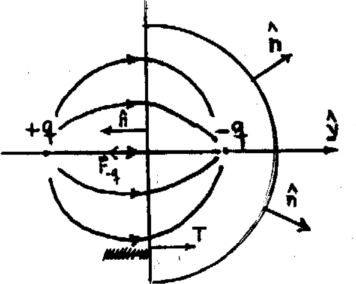
\includegraphics[width=0.4\textwidth]{images/fig_ft1_tensorM1.pdf}	 
	\end{center}
	\caption{}
\end{figure} 

\begin{figure}[htb]
	\begin{center}
	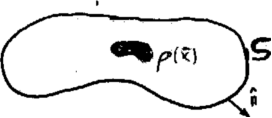
\includegraphics[width=0.4\textwidth]{images/fig_ft1_maxwell.pdf}	 
	\end{center}
	\caption{}
\end{figure} 


\begin{figure}[htb]
	\begin{center}
	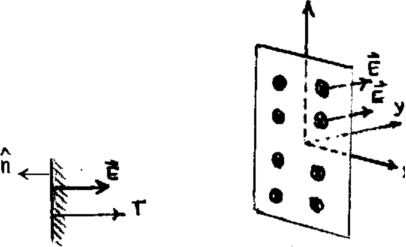
\includegraphics[width=0.4\textwidth]{images/fig_ft1_tensorM2.pdf}	 
	\end{center}
	\caption{}
\end{figure} 

\begin{figure}[htb]
	\begin{center}
	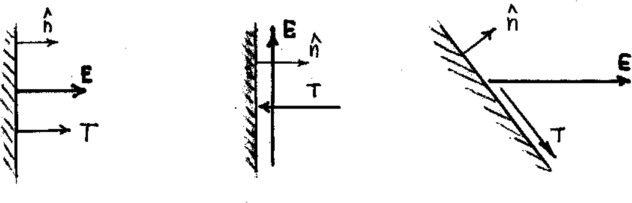
\includegraphics[width=0.4\textwidth]{images/fig_ft1_tensorM3.pdf}	 
	\end{center}
	\caption{}
\end{figure} 

\begin{figure}[htb]
	\begin{center}
	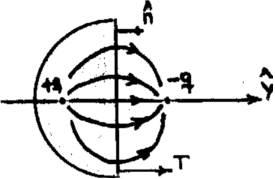
\includegraphics[width=0.4\textwidth]{images/fig_ft1_tensorM4.pdf}	 
	\end{center}
	\caption{}
\end{figure} 

\begin{figure}[htb]
	\begin{center}
	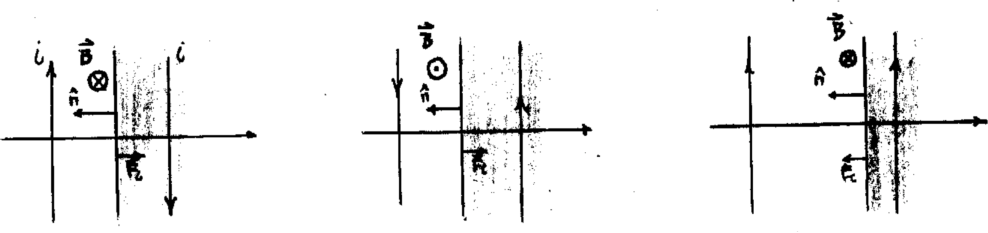
\includegraphics[width=0.4\textwidth]{images/fig_ft1_tensorM5.pdf}	 
	\end{center}
	\caption{}
\end{figure} 



% \bibliographystyle{CBFT-apa-good}	% (uses file "apa-good.bst")
% \bibliography{CBFT.Referencias} % La base de datos bibliográfica

\end{document}
